%%%%%%%%%%%%%%%%%%%%%%%%%%%%%%%%%%%%%%%%%%%%%%%%%%%%%%%%%%%%%%%%%%%%%%%%%%%%%%%%%%%%%%%%%%%%%%%%%
%
% Document:     DM Support Products  product tree
%
%%%%%%%%%%%%%%%%%%%%%%%%%%%%%%%%%%%%%%%%%%%%%%%%%%%%%%%%%%%%%%%%%%%%%%%%%%%%%%
\documentclass{article}
\usepackage{times,layouts}
\usepackage{tikz,hyperref,amsmath}
\usetikzlibrary{positioning,arrows,shapes,decorations.shapes,shapes.arrows}
\usetikzlibrary{backgrounds,calc}
\usepackage[paperwidth=411.99999999999994pt,paperheight=430pt,
left=-2mm,top=3mm,bottom=0mm,right=0mm,
noheadfoot,marginparwidth=0pt,includemp=false,
textwidth=30cm,textheight=50mm]{geometry}
\newcommand\showpage{%
\setlayoutscale{0.5}\setlabelfont{\tiny}\printheadingsfalse\printparametersfalse
\currentpage\pagedesign}
\hypersetup{pdftitle={DM Support Products products }, pdfsubject={Diagram illustrating the
                products in LSST DM Support Products }, pdfauthor={Extracted from MagicDraw}}
\tikzstyle{tbox}=[rectangle,text centered, text width=30mm]
\tikzstyle{wbbox}=[rectangle, rounded corners=3pt, draw=black, top color=blue!50!white,
                    bottom color=white, very thick, minimum height=40pt, inner sep=2pt,
                    text centered, text width=30mm]
\tikzstyle{pbox}=[rectangle, rounded corners=3pt, draw=black, top
 color=yellow!50!white, bottom color=white, very thick,
 minimum height=36pt, inner sep=3pt, text centered, text width=35mm]
\tikzstyle{pline}=[-, thick]
\begin{document}
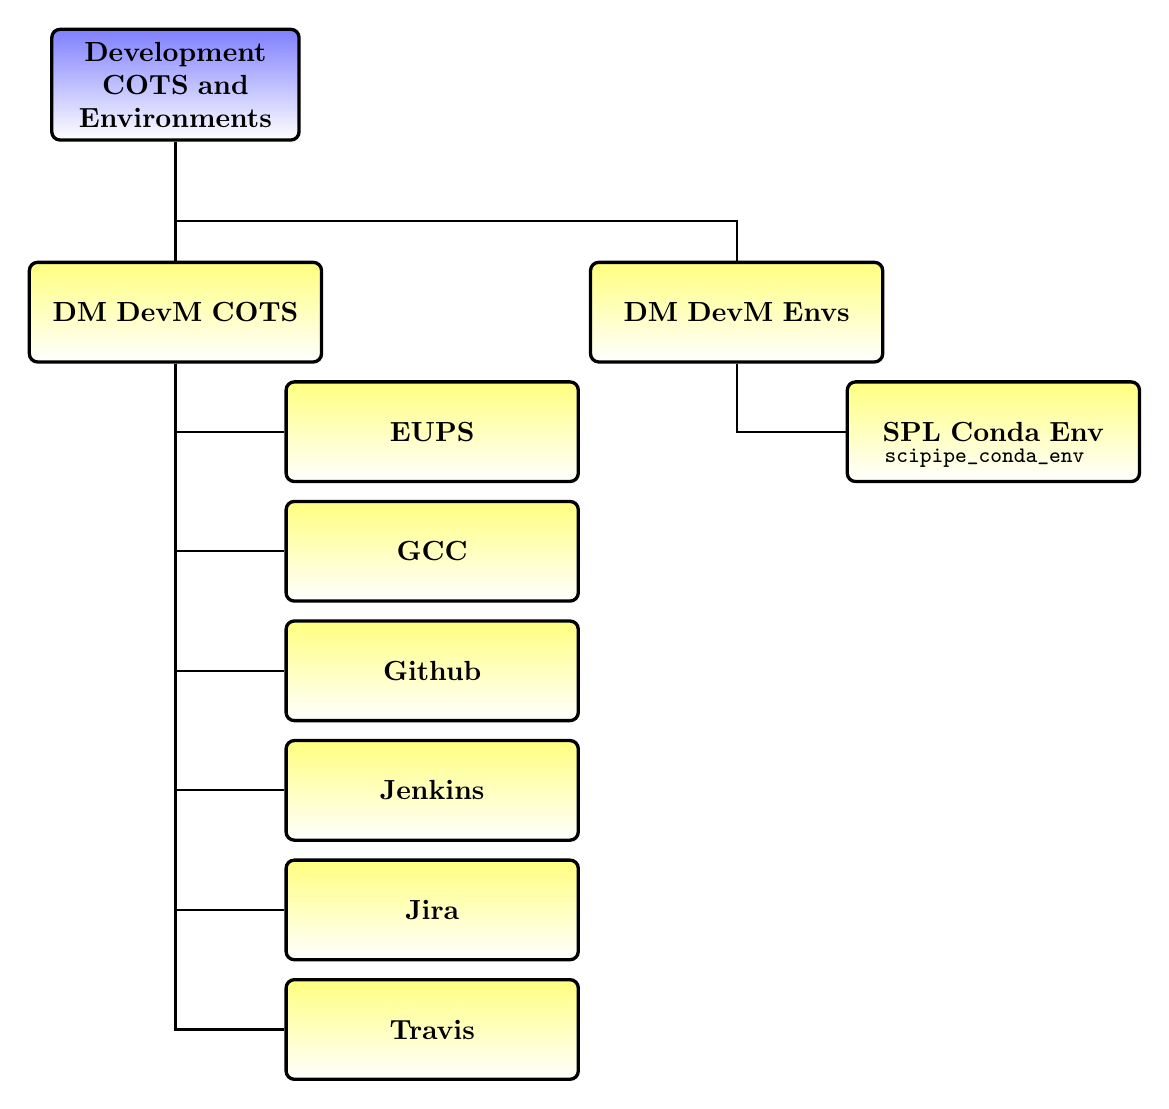
\begin{tikzpicture}[node distance=0mm]


\node (COTSDM) [pbox, 
] {\textbf{DM DevM COTS
} };\node [below right] at (COTSDM.north west) {\footnotesize \color{blue}} ;

\node (EUPS) [pbox,below right=6pt and -14pt of COTSDM] {\textbf{EUPS
} };\node [below right] at (EUPS.north west) {\footnotesize \color{blue}} ;

 \draw[pline] (COTSDM.south) -| ++(0,0) |- (EUPS.west); 
\node (GCC) [pbox,below=6pt of EUPS] {\textbf{GCC
} };\node [below right] at (GCC.north west) {\footnotesize \color{blue}} ;

 \draw[pline] (COTSDM.south) -| ++(0,0) |- (GCC.west); 
\node (GITHUB) [pbox,below=6pt of GCC] {\textbf{Github
} };\node [below right] at (GITHUB.north west) {\footnotesize \color{blue}} ;

 \draw[pline] (COTSDM.south) -| ++(0,0) |- (GITHUB.west); 
\node (JNKNS) [pbox,below=6pt of GITHUB] {\textbf{Jenkins
} };\node [below right] at (JNKNS.north west) {\footnotesize \color{blue}} ;

 \draw[pline] (COTSDM.south) -| ++(0,0) |- (JNKNS.west); 
\node (JRA) [pbox,below=6pt of JNKNS] {\textbf{Jira
} };\node [below right] at (JRA.north west) {\footnotesize \color{blue}} ;

 \draw[pline] (COTSDM.south) -| ++(0,0) |- (JRA.west); 
\node (TRVS) [pbox,below=6pt of JRA] {\textbf{Travis
} };\node [below right] at (TRVS.north west) {\footnotesize \color{blue}} ;

 \draw[pline] (COTSDM.south) -| ++(0,0) |- (TRVS.west); 
\node (DENV) [pbox, 
right=96pt of COTSDM] {\textbf{DM DevM Envs
} };\node [below right] at (DENV.north west) {\footnotesize \color{blue}} ;

\node (SPLCE) [pbox,below right=6pt and -14pt of DENV] {\textbf{SPL Conda Env
} };\node [below right] at (SPLCE.north west) {\footnotesize \color{blue}} ;
\node (SPLCEpkg) [tbox,below=3mm of SPLCE.north] {{\footnotesize \color{black} \begin{verbatim} scipipe_conda_env \end{verbatim} }  };

 \draw[pline] (DENV.south) -| ++(0,0) |- (SPLCE.west); 
\node (DMDC3E) [wbbox, above=43pt of COTSDM]{\textbf{Development COTS and Environments}};
 \draw[pline]   (COTSDM.north) -- ++(0.0,0.5) -| (DMDC3E.south) ; 
 \draw[pline]   (DENV.north) -- ++(0.0,0.5) -| (DMDC3E.south) ; 

\end{tikzpicture}
\end{document}
